\section{Implementation Alignment}\label{impl:v2}

This v2 draft is intended to align the paper model with the protocol that is
now implemented in the repository. The original protocol description remains
the conceptual source, while this section records the concrete implementation
choices that affect safety, finality, latency, and benchmark interpretation.

\subsection{Implemented Quorum Parameters}

The current protocol implementation defines a fixed quorum size of six in
\path{src/algorithm.rs}. The same module defines the implemented
supermajority threshold:
\[
S(x)=x-\left\lfloor \frac{x}{3}\right\rfloor .
\]
For a six-member quorum this gives \(S(6)=4\). The verified path's Byzantine
safety proof uses
\[
F(x)=\left\lfloor \frac{x-1}{3}\right\rfloor
\]
as the maximum Byzantine population that can be tolerated while guaranteeing
honest overlap between two accepted supermajority proofs. Therefore a
six-member quorum can make liveness progress without two slow or absent
members, but the honest-overlap safety proof admits one Byzantine signer in
that six-member quorum. This distinction is important: slow-node tolerance and
Byzantine equivocator tolerance are related, but not identical.

The implemented quorum schedule is deterministic. Nodes are sorted by public
key, optionally shuffled from the epoch seed, and then assigned into a
\(q\)-ary tensor coordinate system. For active validator count \(n\) and
quorum size \(q\), the schedule dimension is
\[
D(n,q)=\max \left(1,\left\lceil \log_q(n)\right\rceil\right).
\]
The ideal tensor capacity is \(q^{D(n,q)}\). Non-ideal network sizes are mapped
into the same deterministic schedule, with overflow validators appended into
existing quorums according to the public ordering. This preserves a common
quorum view across honest validators while allowing the implementation to run
when \(n\) is not exactly a power of \(q\).

Conceptually, a validator occupies a coordinate
\[
    a_i=(a_{i,0},a_{i,1},\ldots,a_{i,D-1}) \in [q]^D .
\]
Each consensus layer moves across one tensor dimension. The local quorum for a
layer consists of validators that share the node's other coordinates and vary
along the active dimension. Earlier protocol drafts used this schedule directly:
for \(n=36\) and \(q=6\), the network formed a \(6 \times 6\) tensor and ran a
row-like round followed by a column-like round. If the first data-spreading
round failed, however, a correct local block could remain trapped at the leaf
of the tree and be lost from that branch.

The 2025--2026 v2 implementation therefore adds deterministic
\emph{prefill dispatch}. Before verified consensus begins, each node sends its
local block to the future contacts that will carry that block through the
remaining tensor layers. In the default single-route profile, the remote
prefill fanout is
\[
P(n,q)=\min \left(n-1,\ (q-1)+(D(n,q)-1)q\right),
\]
or approximately \(Dq\) holders including the source node. The prefill stage
replaces only the first data-spreading consensus round; the later verified
rounds still run and certify the canonical epoch state. With \(q=6\) and
\(D=10\), this means a node sends to \(59\) remote contacts, or \(60\) holders
including itself, even though the tensor capacity is
\(6^{10}=60{,}466{,}176\) validators.

\begin{figure}[h!]
    \centering
    \resizebox{\columnwidth}{!}{
    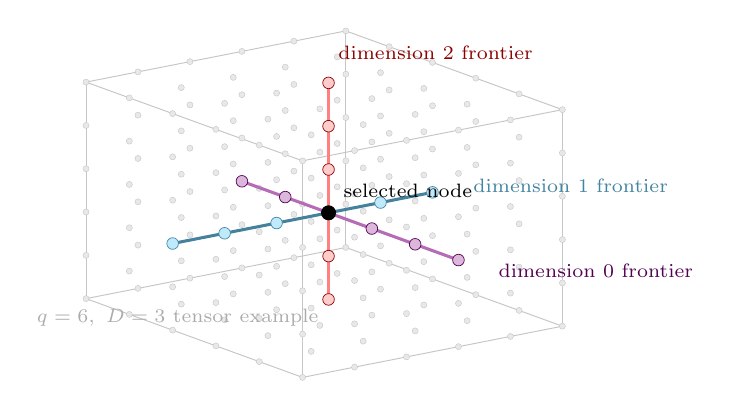
\begin{tikzpicture}[
        x={(0.55cm,-0.20cm)},
        y={(0.66cm,0.13cm)},
        z={(0cm,0.55cm)},
        every node/.style={font=\scriptsize},
        cube edge/.style={gray!45,line width=0.35pt},
        base dot/.style={circle,draw=gray!45,fill=gray!18,line width=0.15pt,minimum size=2.2pt,inner sep=0pt},
        purple dot/.style={circle,draw=violet!65!black,fill=violet!28,line width=0.25pt,minimum size=4.2pt,inner sep=0pt},
        blue dot/.style={circle,draw=cyan!60!black,fill=cyan!25,line width=0.25pt,minimum size=4.2pt,inner sep=0pt},
        red dot/.style={circle,draw=red!55!black,fill=red!20,line width=0.25pt,minimum size=4.2pt,inner sep=0pt},
        selected dot/.style={circle,draw=black,fill=black,minimum size=5pt,inner sep=0pt},
        purple line/.style={violet!58,line width=1.1pt},
        blue line/.style={cyan!58!black,line width=1.1pt},
        red line/.style={red!50,line width=1.1pt}
    ]
        \def\sx{2}
        \def\sy{3}
        \def\sz{2}

        \draw[cube edge] (0,0,0) -- (5,0,0) -- (5,5,0) -- (0,5,0) -- cycle;
        \draw[cube edge] (0,0,5) -- (5,0,5) -- (5,5,5) -- (0,5,5) -- cycle;
        \draw[cube edge] (0,0,0) -- (0,0,5);
        \draw[cube edge] (5,0,0) -- (5,0,5);
        \draw[cube edge] (5,5,0) -- (5,5,5);
        \draw[cube edge] (0,5,0) -- (0,5,5);

        \foreach \x in {0,...,5} {
            \foreach \y in {0,...,5} {
                \foreach \z in {0,...,5} {
                    \node[base dot] at (\x,\y,\z) {};
                }
            }
        }

        \draw[purple line] (0,\sy,\sz) -- (5,\sy,\sz);
        \draw[blue line] (\sx,0,\sz) -- (\sx,5,\sz);
        \draw[red line] (\sx,\sy,0) -- (\sx,\sy,5);

        \foreach \x in {0,...,5} {
            \node[purple dot] at (\x,\sy,\sz) {};
        }
        \foreach \y in {0,...,5} {
            \node[blue dot] at (\sx,\y,\sz) {};
        }
        \foreach \z in {0,...,5} {
            \node[red dot] at (\sx,\sy,\z) {};
        }
        \node[selected dot,label={[font=\scriptsize]above right:selected node}] at (\sx,\sy,\sz) {};

        \node[text=violet!65!black,anchor=west] at (5.7,\sy,\sz) {dimension 0 frontier};
        \node[text=cyan!60!black,anchor=west] at (\sx,5.6,\sz) {dimension 1 frontier};
        \node[text=red!55!black,anchor=west] at (\sx,\sy,5.7) {dimension 2 frontier};
        \node[anchor=west,text=gray!65] at (-0.4,-0.8,-0.4) {\(q=6,\ D=3\) tensor example};
    \end{tikzpicture}
    }
    \caption{Tensor quorum geometry for \(q=6\) and \(D=3\). The selected node is placed in a \(6 \times 6 \times 6\) coordinate tensor. Each pastel line fixes the selected node's coordinates in all but one dimension; the free dimension is one future quorum frontier. In v2, prefill dispatch sends the local block to the union of these future contacts before verified consensus skips the old first data-spreading round.}
    \label{fig:tensor_prefill_cube}
\end{figure}


\subsection{Trusted and Verified Paths}

The implementation now distinguishes two execution paths:

\begin{description}
\item[Trusted path] assumes known-safe operators and uses dispatch-only
propagation. This path models private or permissioned environments where
operators do not intentionally equivocate.
\item[Verified path] uses the full message sequence: dispatch, echo,
verification, proposal, and commit. Votes are counted by distinct current
validator identities, and each signed message is bound to the epoch, nonce,
round, message kind, sender identity, and body being admitted.
\end{description}

The epoch benchmark binary models these paths separately. For a two-layer
\(q=6\) topology, the legacy trusted path has two data-moving stages, while
the legacy verified path has ten proof-bearing network stages. With v2 prefill
dispatch enabled, the first data-spreading verified round is replaced by one
availability hop, so the same two-layer topology uses one prefill hop plus one
five-message verified round.

\subsection{Default Trustless Epoch Ordering}

The default trustless build enables fair block ordering, exposed in code under
the fair-block-ordering compile-time feature. This feature is
consensus-affecting: it changes the
domain-separated epoch block tree from raw block-hash ordering to fair-order
commitments. The active profile is labeled
sha256+fair-block-ordering and is also encoded with a stable numeric
feature code. Honest validators include the same feature-code byte sequence in
the protocol hash namespace, so mixed raw-order and fair-order fleets reject
one another before attempting to finalize an epoch.

Fair ordering is applied after blocks and transactions have entered the
accepted set. It does not allow a node to make invalid data valid, and it does
not change the quorum threshold. Instead, it derives an epoch-local ordering
key from the canonical block transcript and the total transaction population.
This prevents ledger-style applications from relying on raw hash order as a
front-running surface. Explicit raw block-hash ordering remains available only
for legacy or private compatibility builds that disable default features.

\subsection{Runtime Reconciliation and Membership}

The protocol code now contains explicit runtime repair and reconnect behavior.
Dropped nodes do not re-enter merely by becoming reachable. A reconnecting node
must ping active peers, obtain a catch-up proof for the current canonical state,
and receive an admission supermajority. In trustless mode, these ping,
catch-up, and admission thresholds are clamped to the same supermajority rule
used elsewhere in the verified path. Duplicate votes, stale proofs, replayed
evidence, and identity changes are counted as telemetry but do not increase the
admission count.

If summary repair cannot find a certified supermajority for an epoch hash, the
simulator falls back to signed block-set reconciliation. The reconciliation
path rebuilds the candidate epoch from signed manifests and requires
supermajority agreement before admitting the result as canonical. These
behaviors are implemented in \path{crates/blossom-sim/src/epoch.rs} and are
covered by deterministic scenario tests.

\subsection{Bounded Awaits and Round-Skip Evidence}

The v2 implementation separates a slow validator from a Byzantine validator.
A node may observe future-round progress and assist that future round, but only
through evidence bound to the current epoch, nonce, source round, target round,
and certified data manifest. The protocol helper in \path{src/round_skip.rs}
defines signed round-skip votes and certificates that count only distinct
current-validator identities under the same supermajority rule used by the
verified path.

The first fanout round is a data-availability boundary. If that round is
skipped before a node's local block has entered the dissemination tree, the
local block is dropped from the assisted future branch. If a later round is
skipped after first fanout, the block is not dropped by default; it is carried
forward by the certified manifest and remains eligible for repair and
reconciliation. The manifest records per-block replica holders, so repair can
reconstruct the full canonical data set from distributed replicas without
requiring one peer to already hold the entire set immediately after first
fanout. Data-bearing future-round votes require validation of the future body
and parent data chain before they can contribute to advancement.

\subsection{Telemetry and Observation}

The v2 implementation embeds protocol telemetry and exports spans to the
observer service in \path{crates/blossom-observer}. The observer is outside the
measured node hot path, but the emitting cost inside each node is part of the
runtime overhead. The current benchmark target is to preserve the telemetry
overhead as an explicit protocol cost while keeping observer analysis separate
from node finality measurements.

\subsection{Benchmark Interpretation}

The benchmark results should be read as implementation-aligned models, not as
proofs that a deployment's network interface can sustain the required load. For
\(n=36\), \(q=6\), and maximum-size blocks under the current frame limit, the
model sends roughly the all-to-all lower-bound amount of full payload data. The
remaining performance question is therefore dominated by the number of network
stages, the supermajority latency ceiling, per-node bandwidth, and the cost of
local verification.
